\documentclass{article}
\usepackage{listings}
\usepackage{ctex}
\usepackage{graphicx}
\usepackage[a4paper, body={18cm,22cm}]{geometry}
\usepackage{amsmath,amssymb,amstext,wasysym,enumerate,graphicx,caption,subfigure}
\usepackage{float,abstract,booktabs,indentfirst,amsmath}
\usepackage{array}
\usepackage{booktabs} %调整表格线与上下内容的间隔
\usepackage{multirow}
\usepackage{url}
\usepackage{diagbox}
\renewcommand\arraystretch{1.4}
\usepackage{indentfirst}
\setlength{\parindent}{2em}
\usepackage{listings}
\usepackage{xcolor}
\lstset{
	numbers=left, 
	numberstyle= \tiny, 
	keywordstyle= \color{ blue!70},
	commentstyle= \color{red!50!green!50!blue!50}, 
	frame=shadowbox, % 阴影效果
	rulesepcolor= \color{ red!20!green!20!blue!20} ,
	escapeinside=``, % 英文分号中可写入中文
	xleftmargin=2em,xrightmargin=2em, aboveskip=1em,
	basicstyle=\footnotesize,
	framexleftmargin=2em
} 


\geometry{left=2.8cm,right=2.2cm,top=2.5cm,bottom=2.5cm}
%\geometry{left=3.18cm,right=3.18cm,top=2.54cm,bottom=2.54cm}

\graphicspath{{figures/}}

\title{\heiti 数字电路实验报告 }

\begin{document}
	\vspace*{1cm}
	
	\begin{figure}[h]
		\centering
		
\includegraphics[scale=1.0]{xh.jpg}
	\end{figure}

	\vspace*{0.5cm}
	
	\begin{center}
		\Huge{\textbf{数字电路实验报告}}
	\end{center}
	
	\vspace{5cm}
	
	\begin{table}[h]
		\centering
		\begin{Large}
			\begin{tabular}{p{3cm} p{7cm}<{\centering}}
				实验题目: &  Logisim 入门     \\ \cline{2-2}
				学生姓名:      & 孔浩宇   \\ \cline{2-2}
				学生学号: & PB20000113 \\ \cline{2-2}
				完成日期:       & 2022/10/13 \\ \cline{2-2}
			\end{tabular}
		\end{Large}		
	\end{table}
	\newpage
    \section{实验题目}
        \subsection*{\qquad Logisim 入门}

    \section{实验目的}
        \subsection*{\qquad (1)能够自行搭建 Logisim 实验环境}
        \subsection*{\qquad (2)熟悉 Logisim 的各种基础器件和基本操作}
        \subsection*{\qquad (3)能够使用 Logisim 搭建组合逻辑电路并进行仿真}
        \subsection*{\qquad (4)能够使用封装子电路并进行电路设计}
    
    \section{实验环境}
        \subsection*{\qquad (1) PC 一台:Windows 操作系统/Java 运行环境(jre)}
        \subsection*{\qquad (2) Logisim 仿真工具 (vesion 2.7.1)}
    
    \section{实验过程}
        \subsection*{Step 1:获取Logisim实验环境}
		\begin{enumerate}
			\item [$1^\circ$]在 vlab.ustc.edu.cn 网站依次点击
			:“使用文档”—>“资源下载”即可进入下载界面。
			\begin{figure}[H]
				\centering
				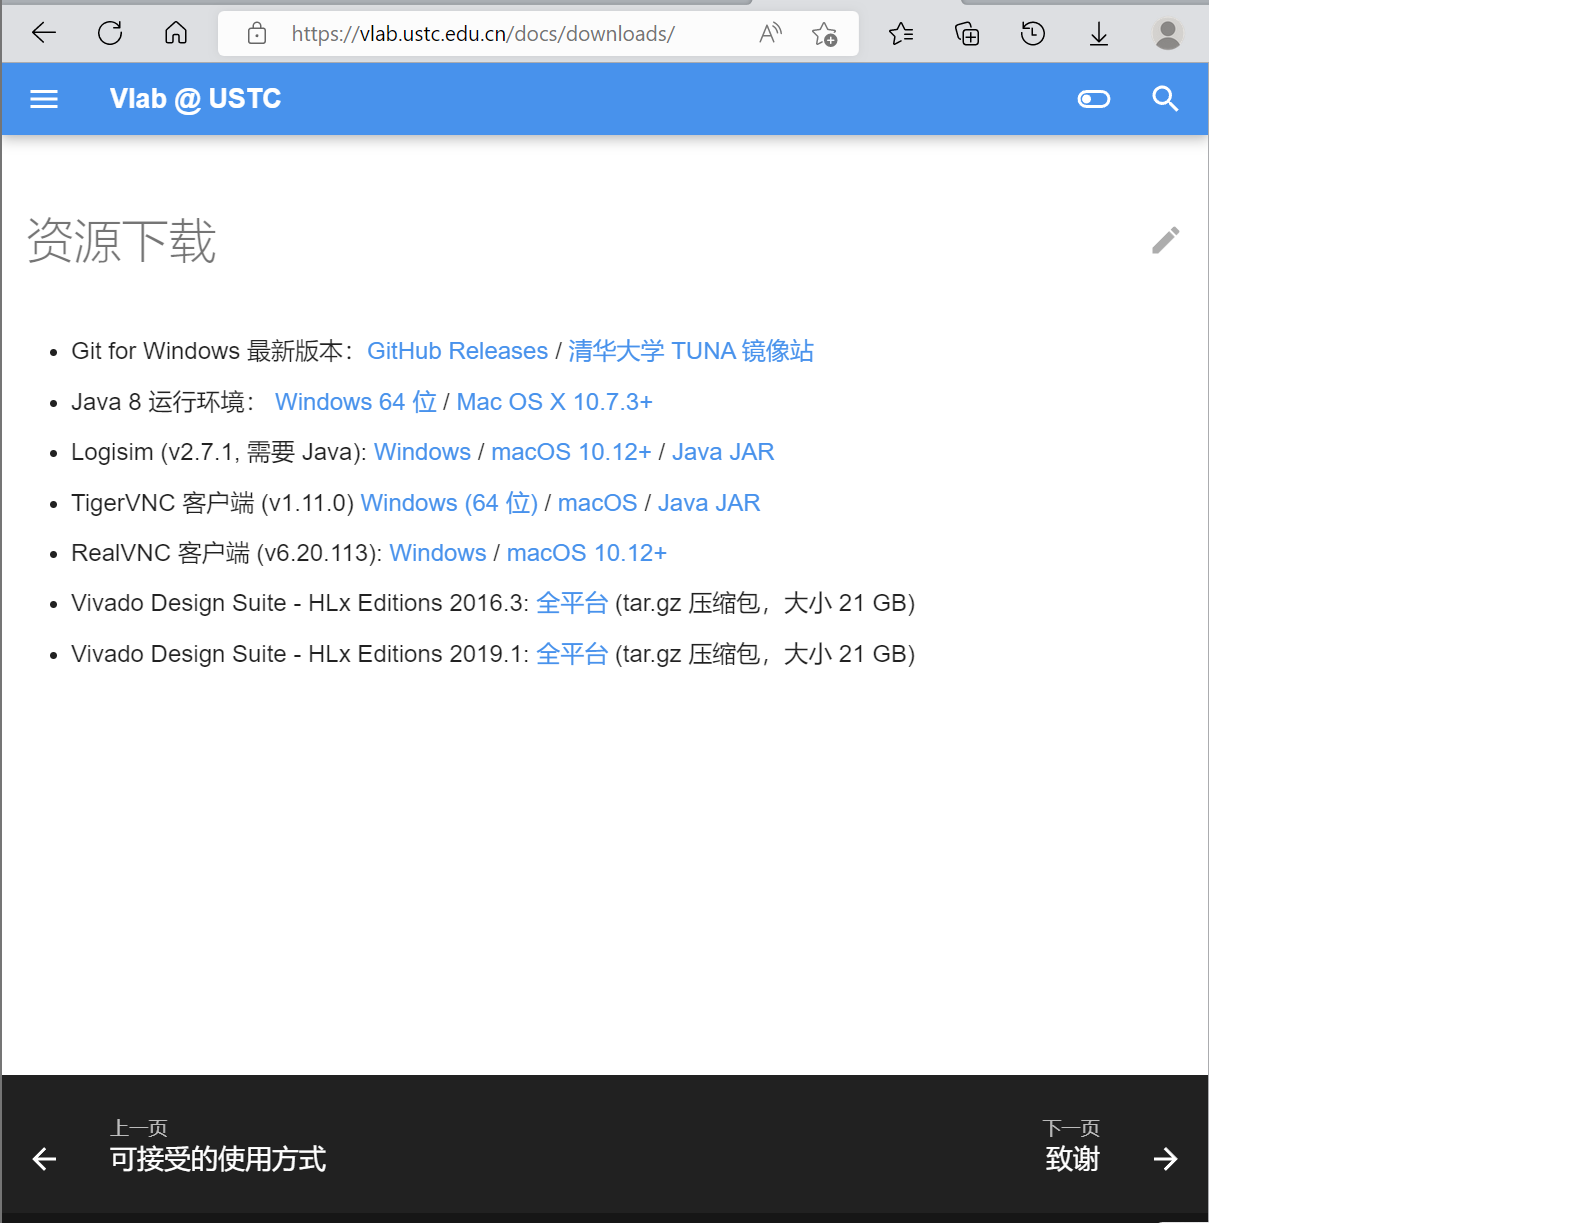
\includegraphics[scale=0.4]{b-0.png}
			\end{figure}
			\item [$2^\circ$]下载与用户操作系统相匹配的 jre 软件和 logisim。
			\begin{figure}[H]
				\centering
				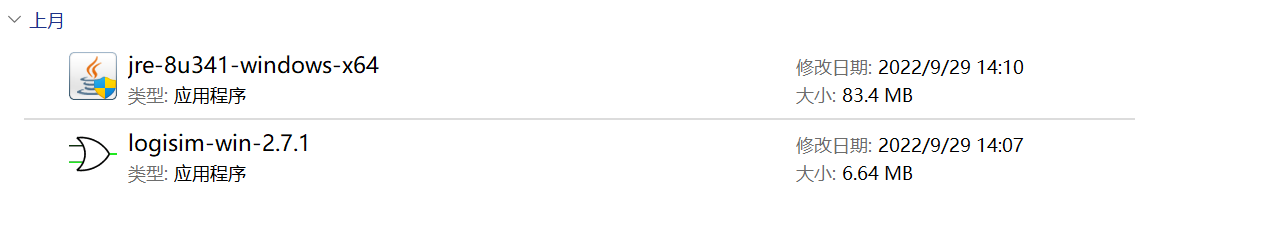
\includegraphics[scale=0.6]{b-1.png}
			\end{figure}
		\end{enumerate}
		\subsection*{Step 2:熟悉Logisim界面}
			\begin{figure}[H]
					\centering
					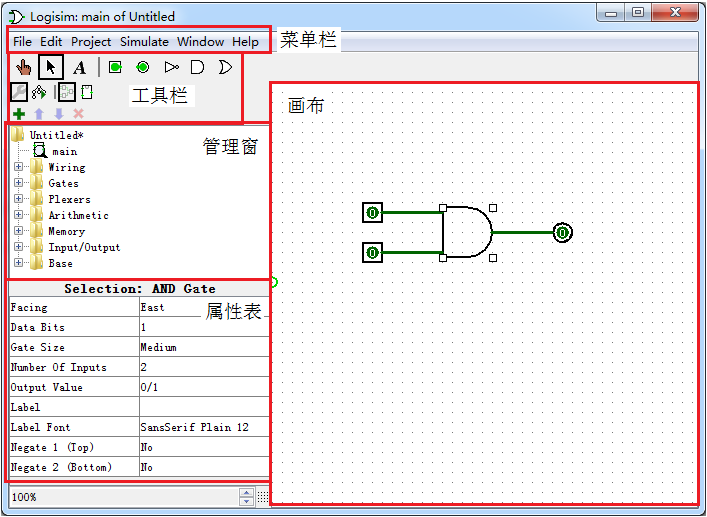
\includegraphics[scale=0.8]{b-2.png}
				\end{figure}
		\subsection*{Step 3:熟悉Logisim基本操作}
		\begin{figure}[H]
			\centering
			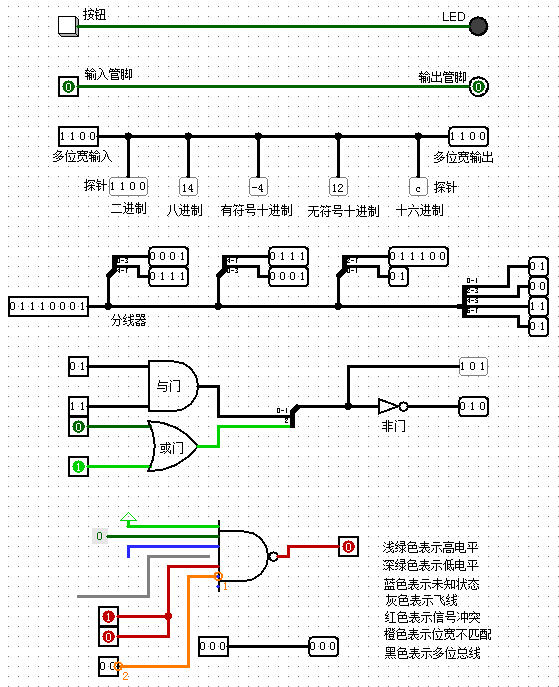
\includegraphics[scale=0.8]{b-3.png}
		\end{figure}
		\begin{figure}[H]
			\centering
			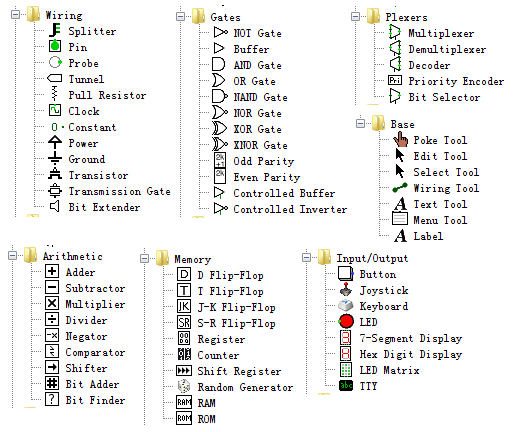
\includegraphics[scale=0.8]{b-4.png}
		\end{figure}
		\subsection*{Step 4:模块封装}
		\begin{enumerate}
			\item [(a)]首先完成半加器add的设计。
			\begin{figure}[H]
				\centering
				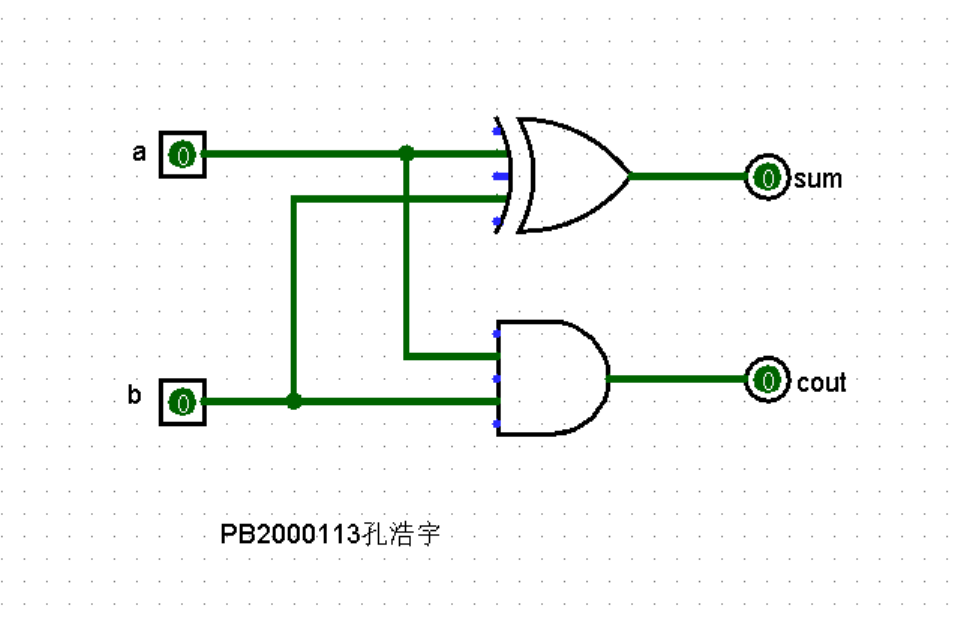
\includegraphics[scale=0.7]{b-5.png}
			\end{figure}
			\item [(b)]对add进行电路封装并编辑。
			\begin{figure}[H]
				\centering
				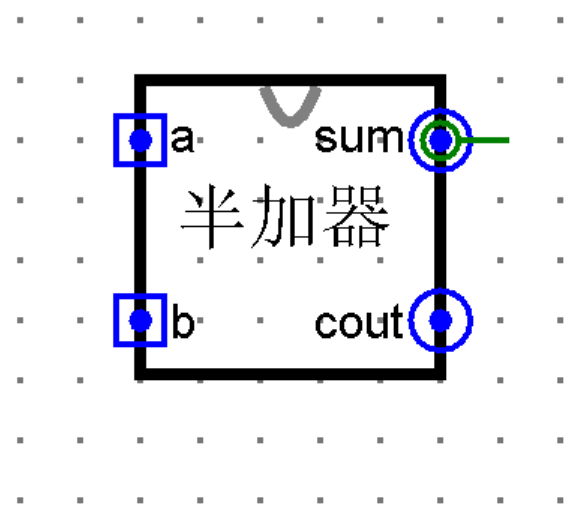
\includegraphics[scale=0.7]{b-6.png}
			\end{figure}
			\item [(c)]在其他电路文件里使用该模块。
			\begin{figure}[H]
				\centering
				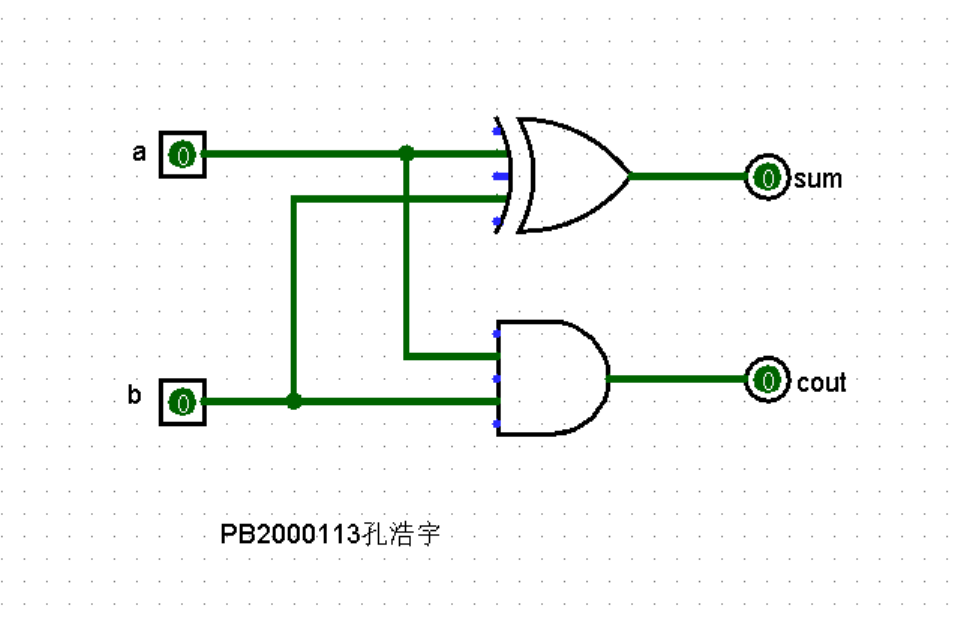
\includegraphics[scale=0.8]{b-5.png}
			\end{figure}
		\end{enumerate}
    \section{实验练习}
		\subsection*{题目1.}使用合适分辨率的 LED 点阵显示出自己的姓名。
		\begin{figure}[H]
			\centering
			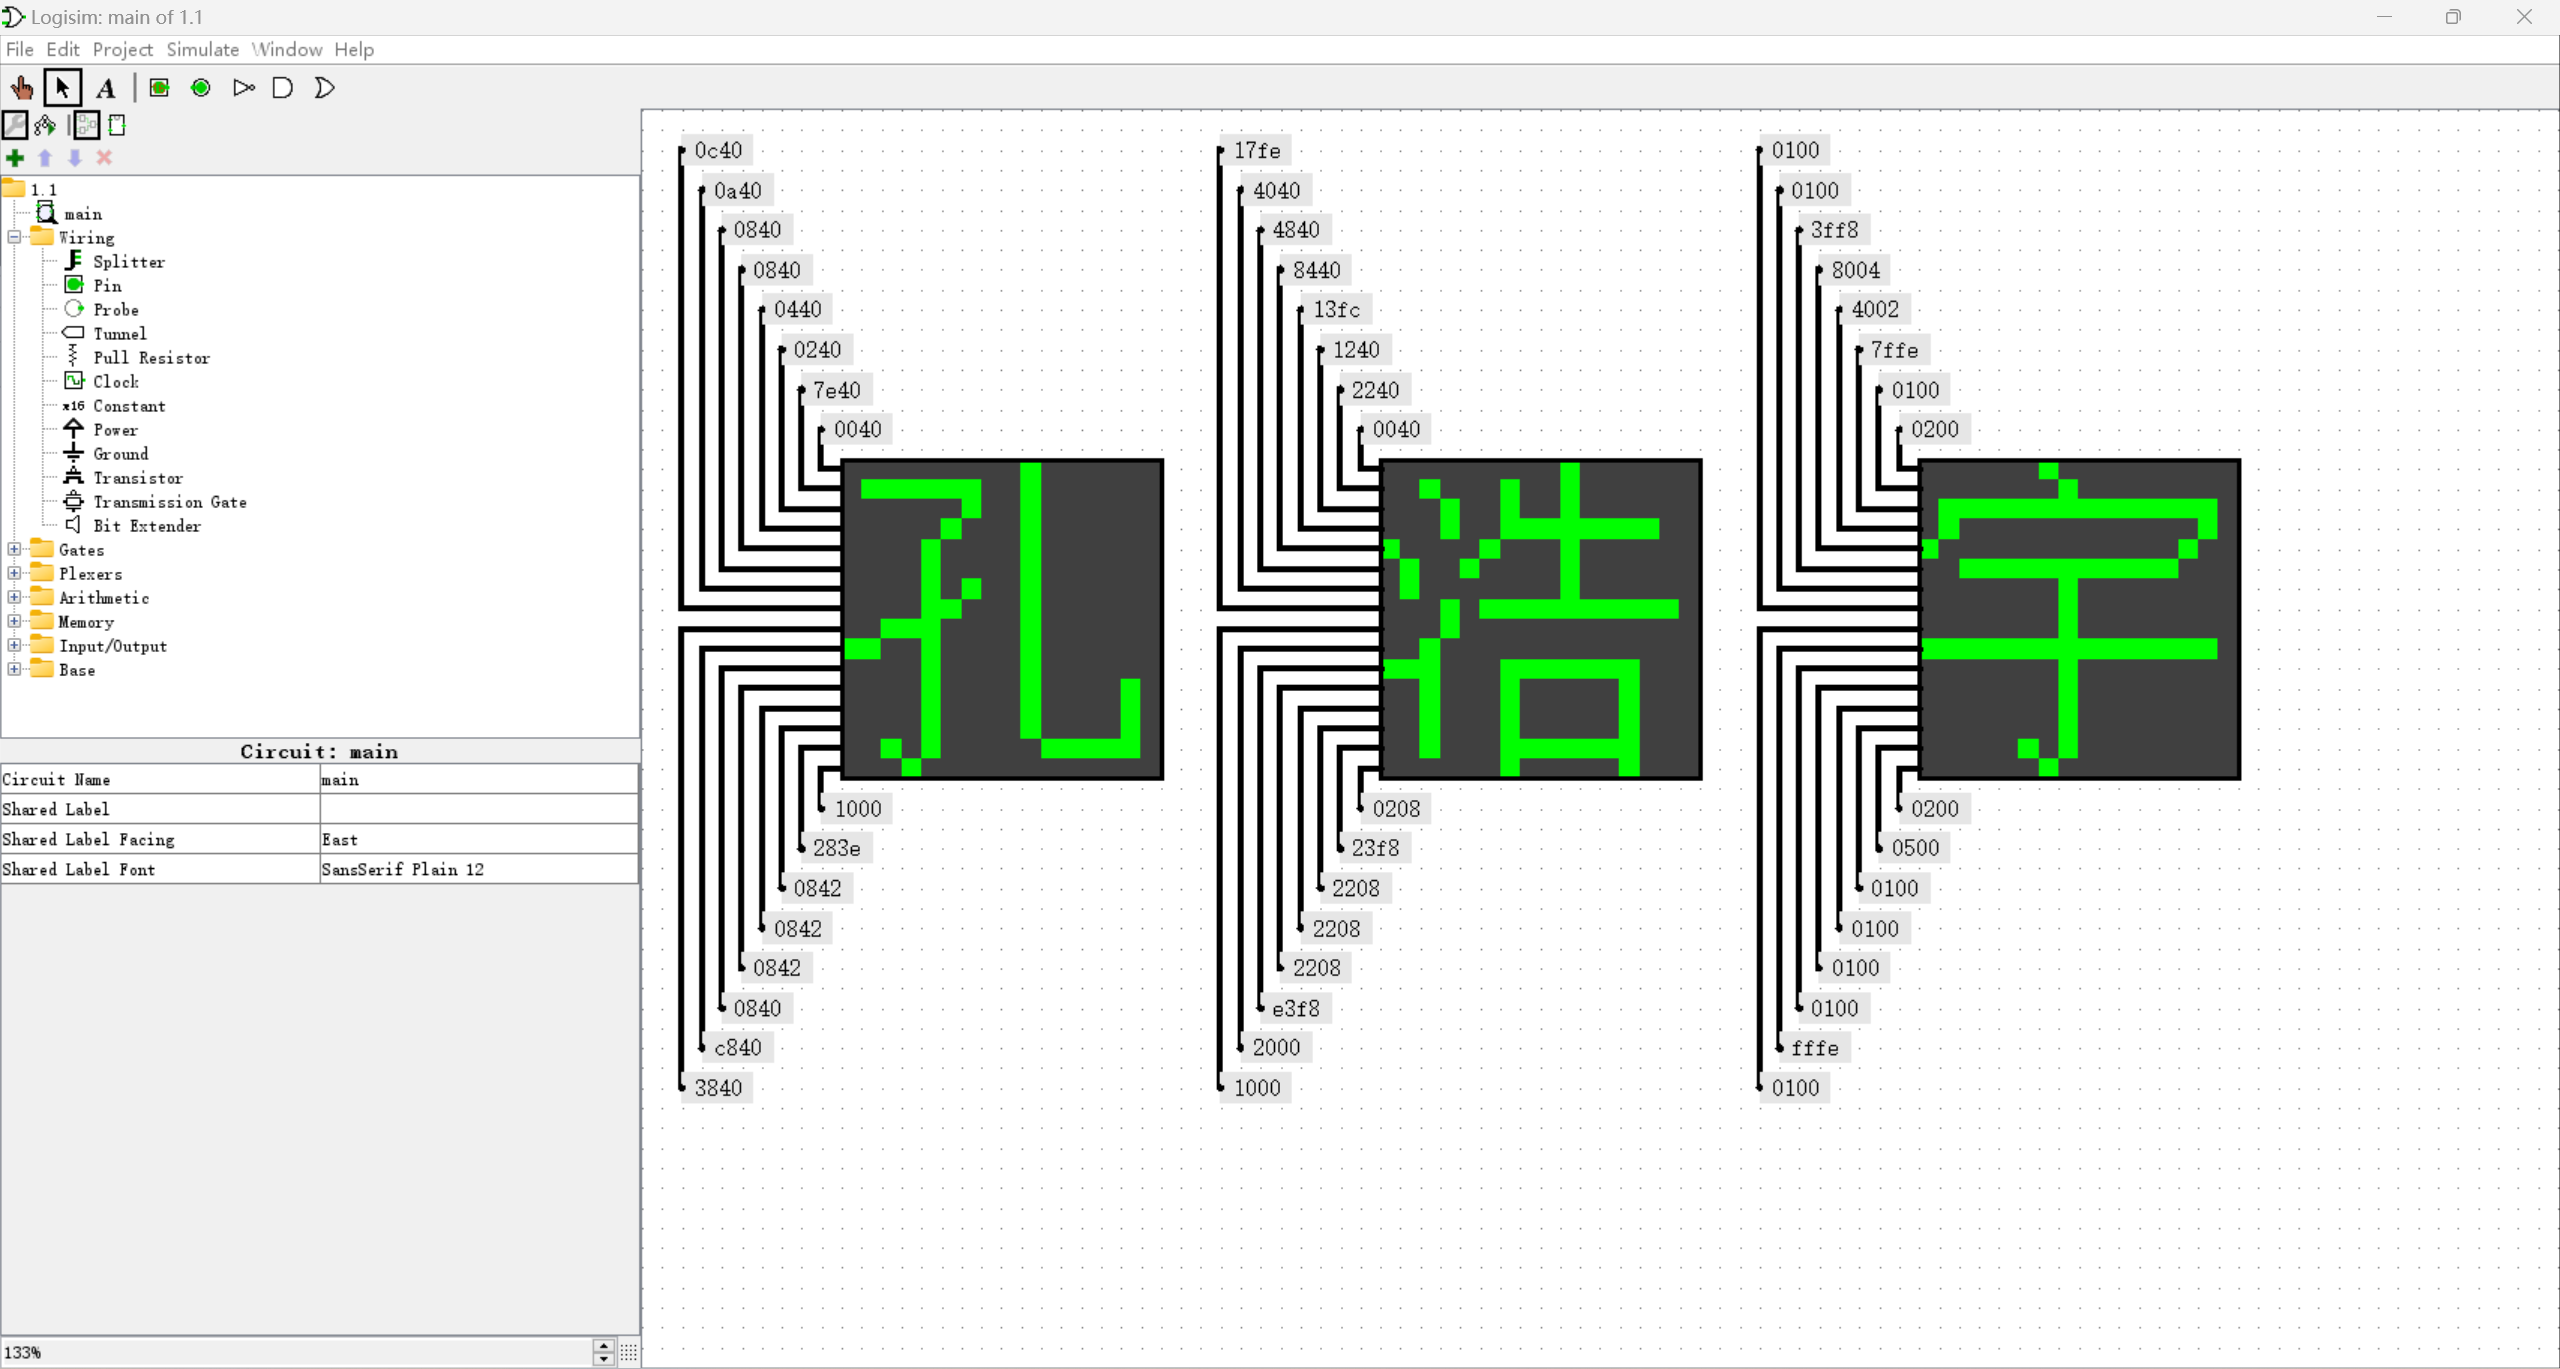
\includegraphics[scale=0.16]{1-1.png}
		\end{figure}
		\subsection*{题目2.}用若干个共阴极七段数码管显示出自己的学号。
		\begin{figure}[H]
			\centering
			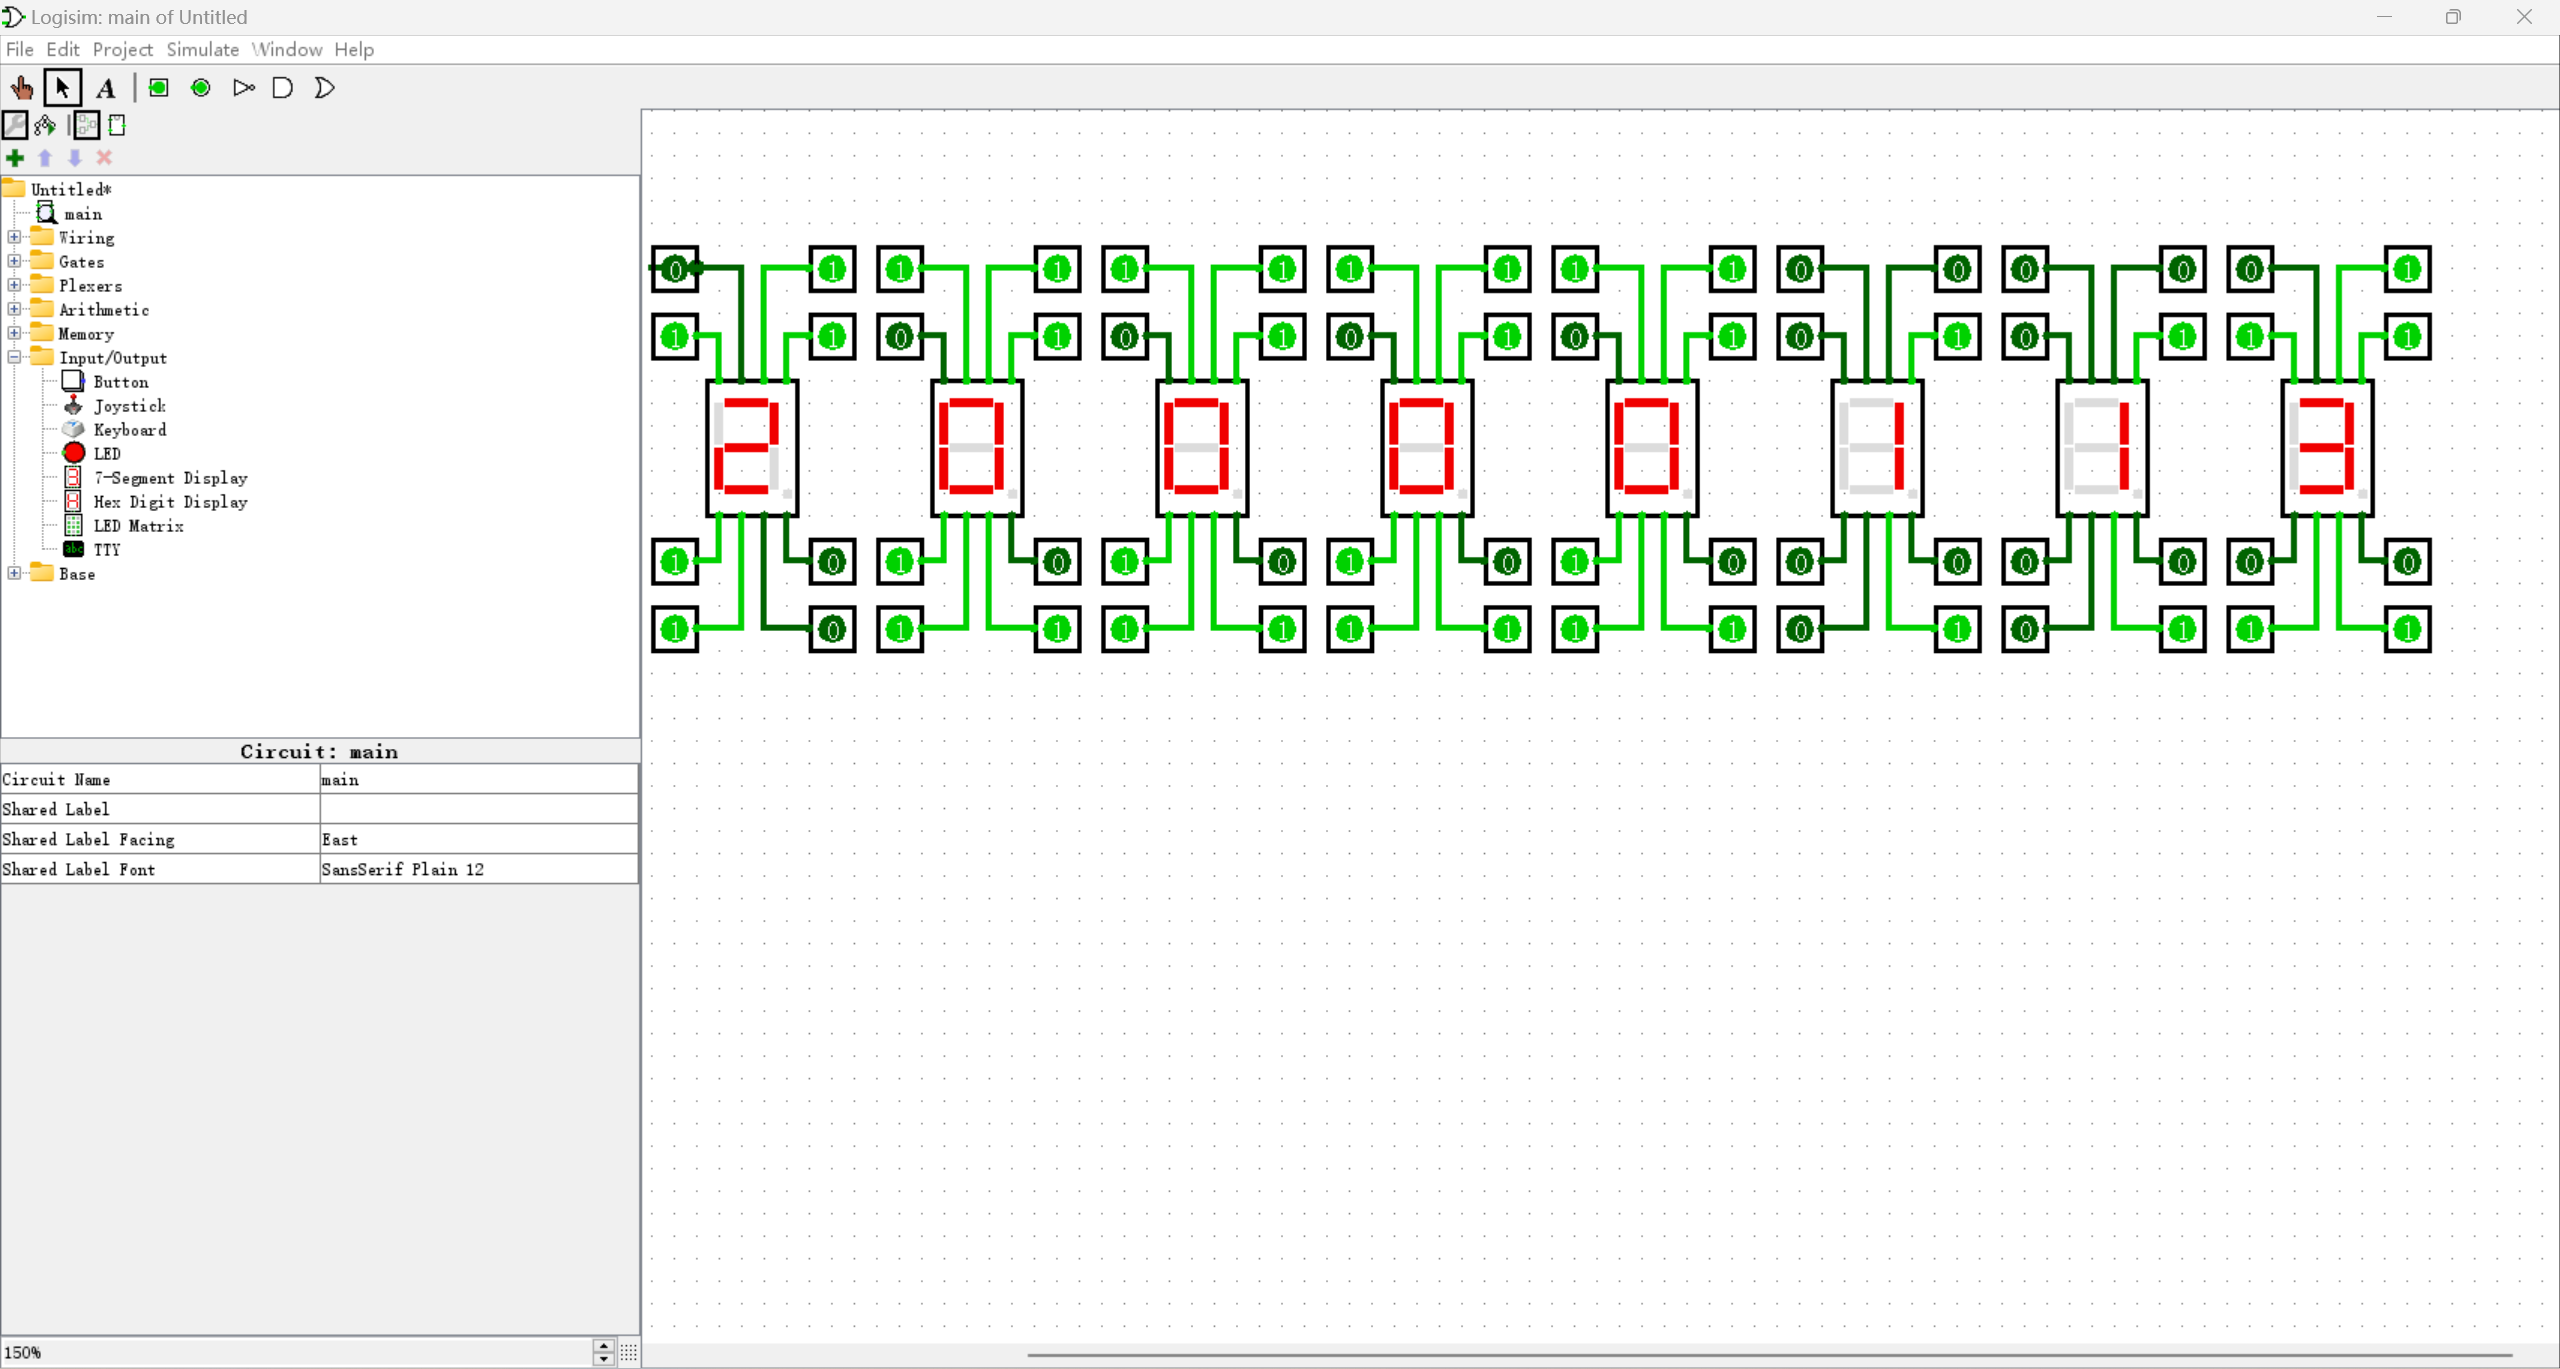
\includegraphics[scale=0.18]{1-2.png}
		\end{figure}
		\subsection*{题目3.}如下图所示,是用晶体管搭出来的三个逻辑门,试分析其行为特
		性,判定各自为哪种逻辑门。用同样的方式搭建与非、或非门。
		\begin{figure}[htbp]
			\centering
			\begin{minipage}{0.49\linewidth}
				\centering
				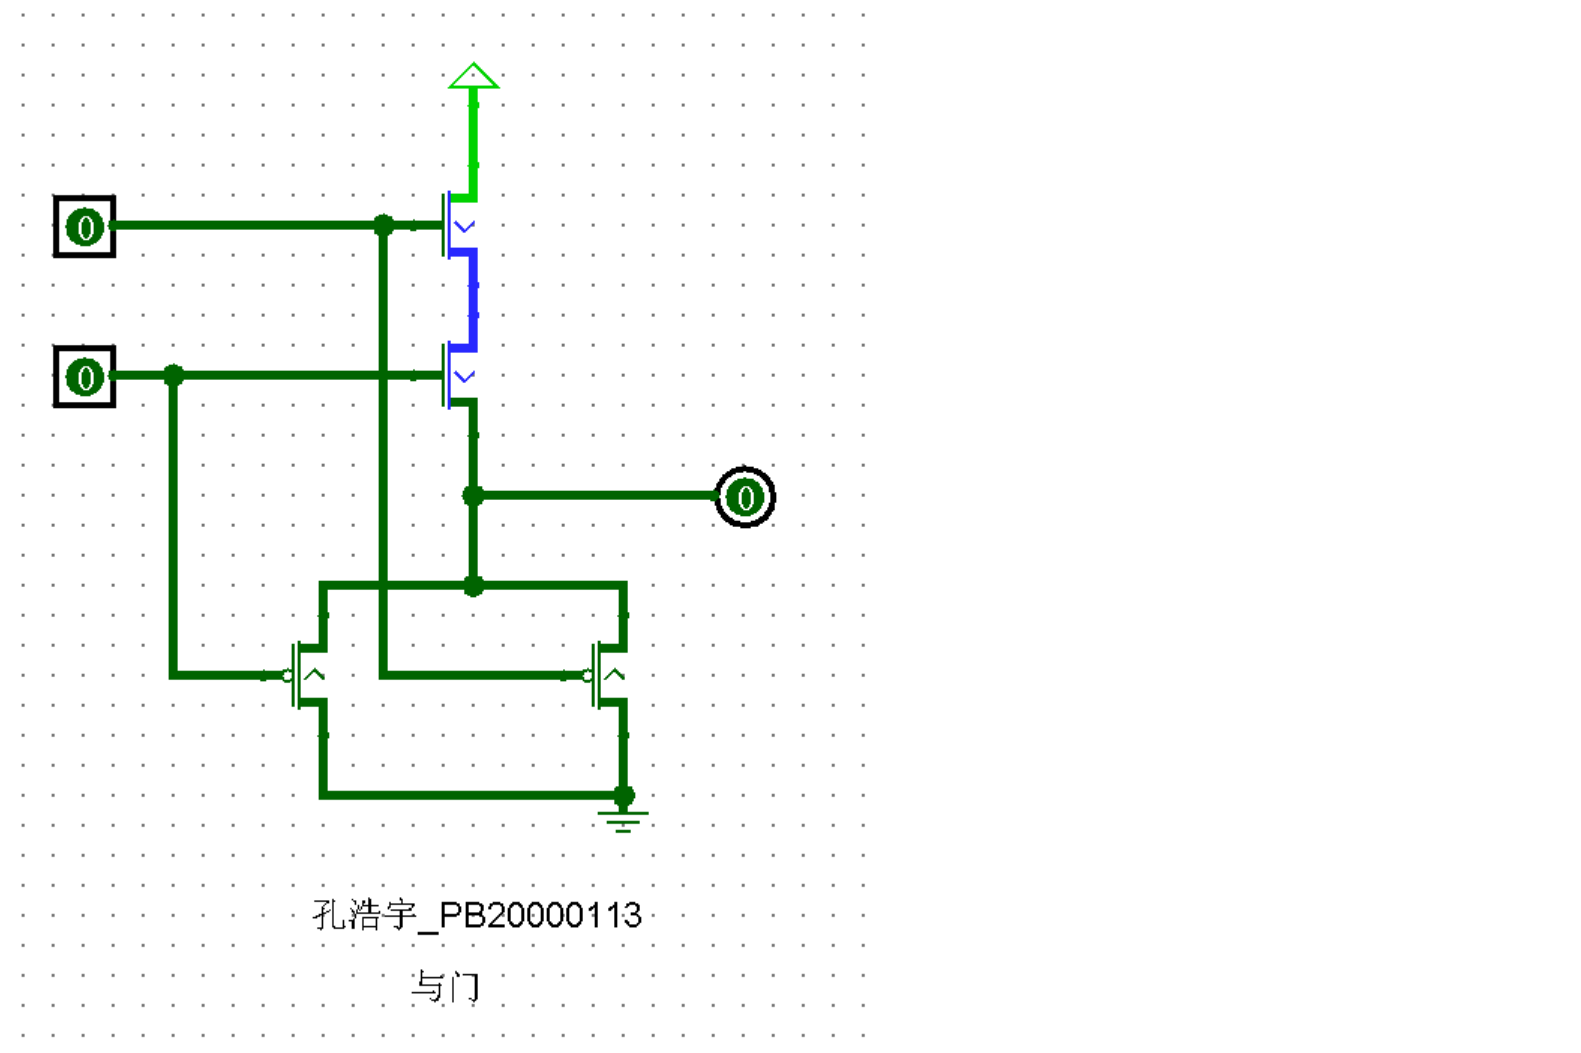
\includegraphics[scale=0.5]{1-3-1.png}
			\end{minipage}
			\begin{minipage}{0.49\linewidth}
				\centering
				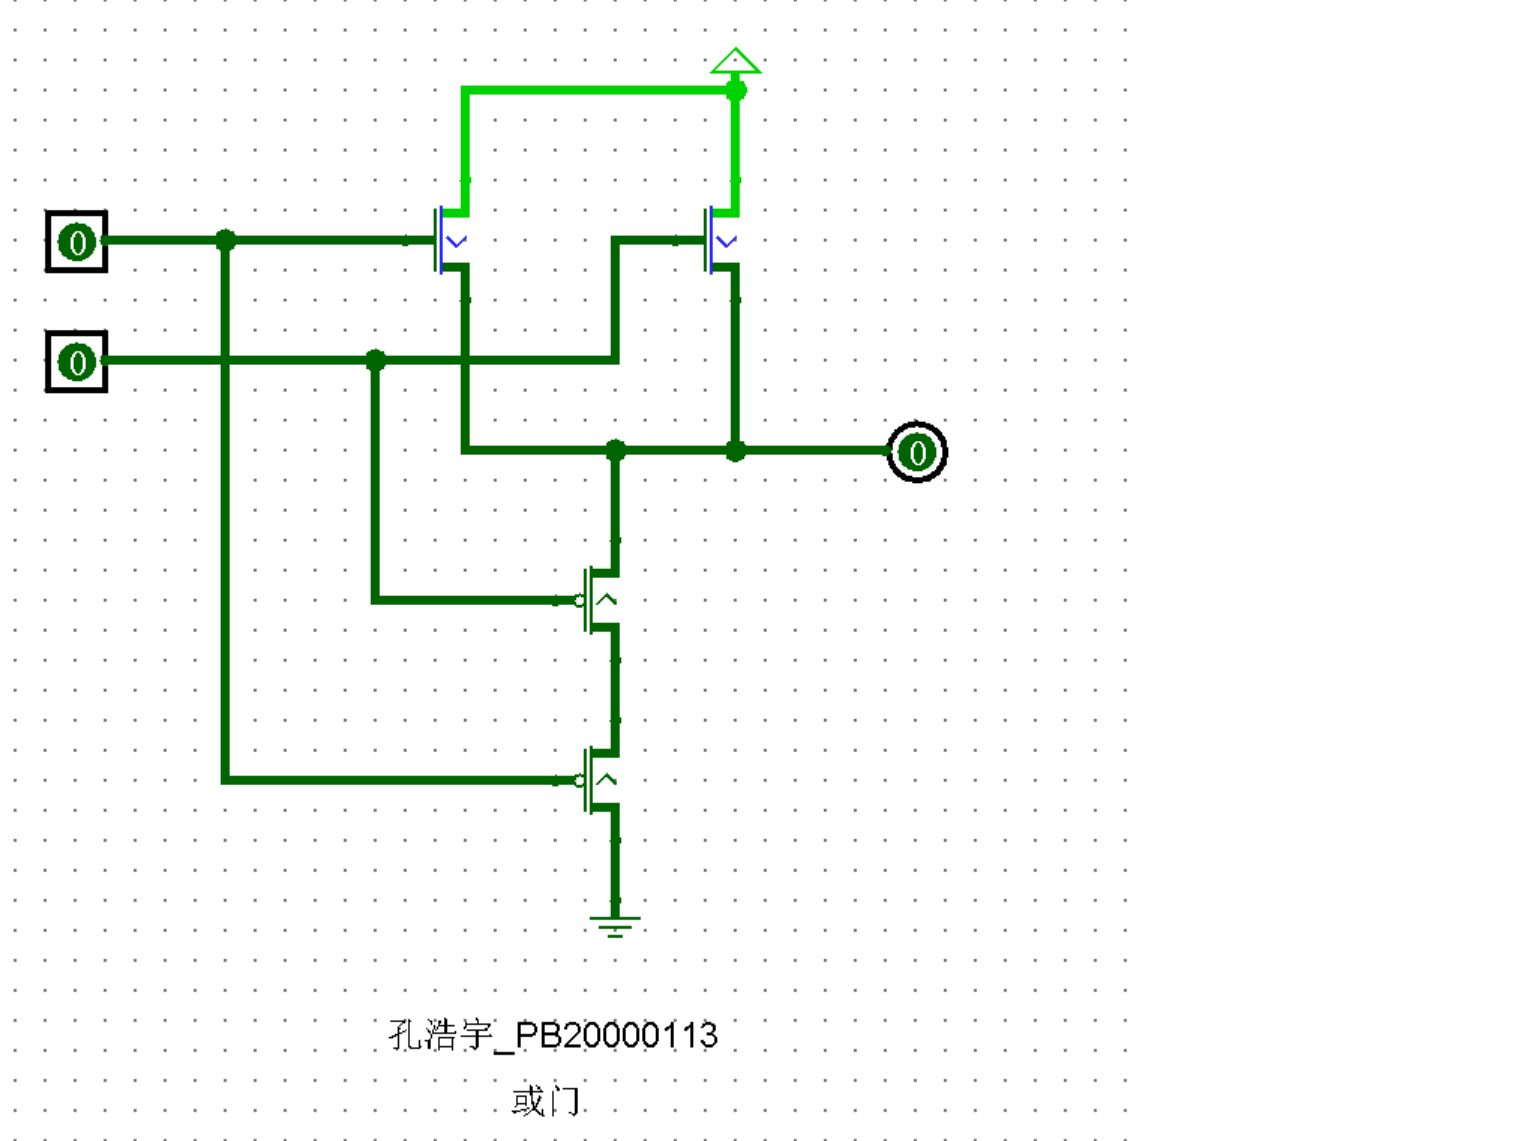
\includegraphics[scale=0.5]{1-3-2.png}
			\end{minipage}
		\end{figure}
		\clearpage
		\begin{figure}[htbp]
			\centering
			\begin{minipage}{0.49\linewidth}
				\centering
				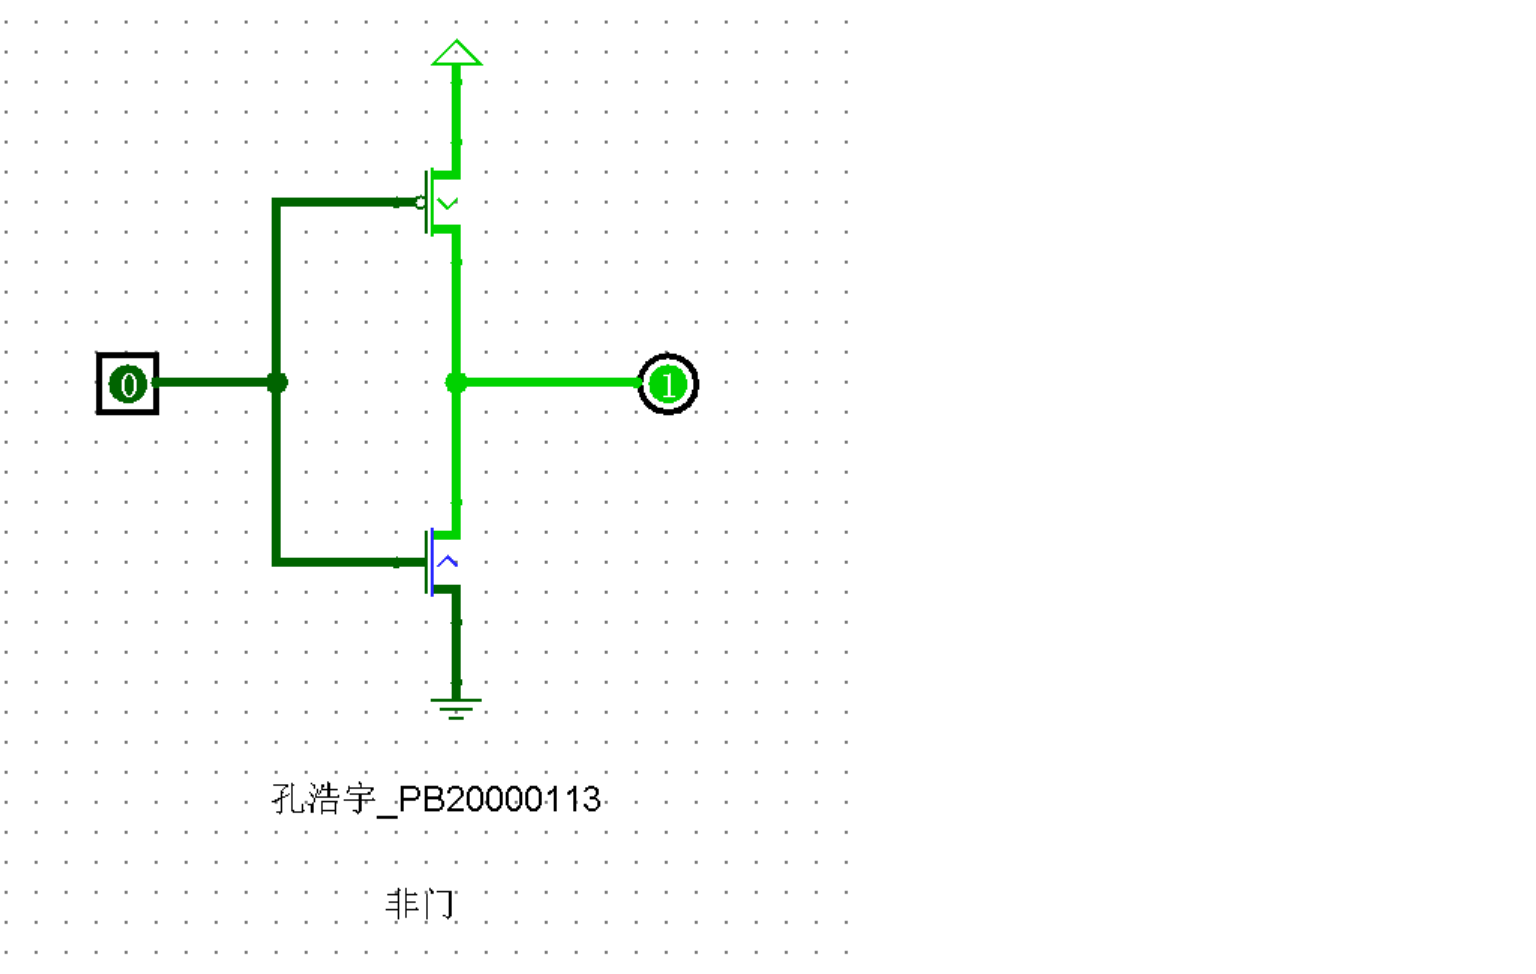
\includegraphics[scale=0.5]{1-3-3.png}
			\end{minipage}
			\begin{minipage}{0.49\linewidth}
				\centering
				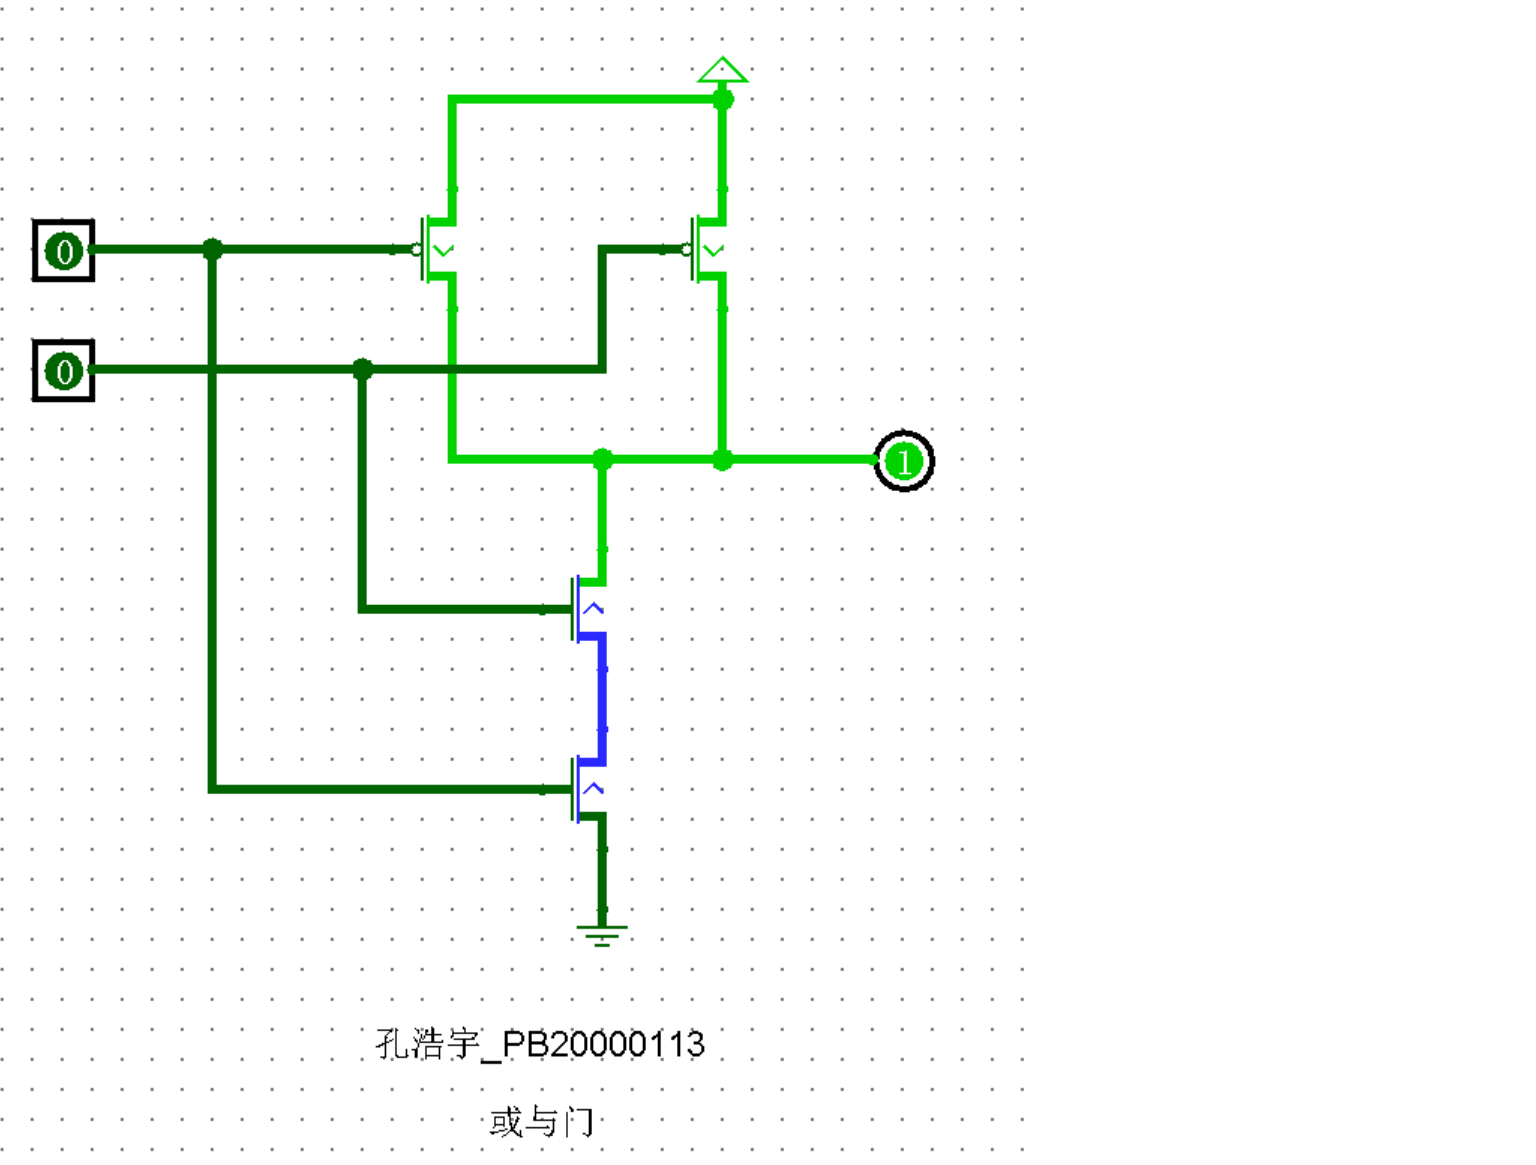
\includegraphics[scale=0.5]{1-3-4.png}
			\end{minipage}
		\end{figure}
		\begin{figure}[H]
			\centering
			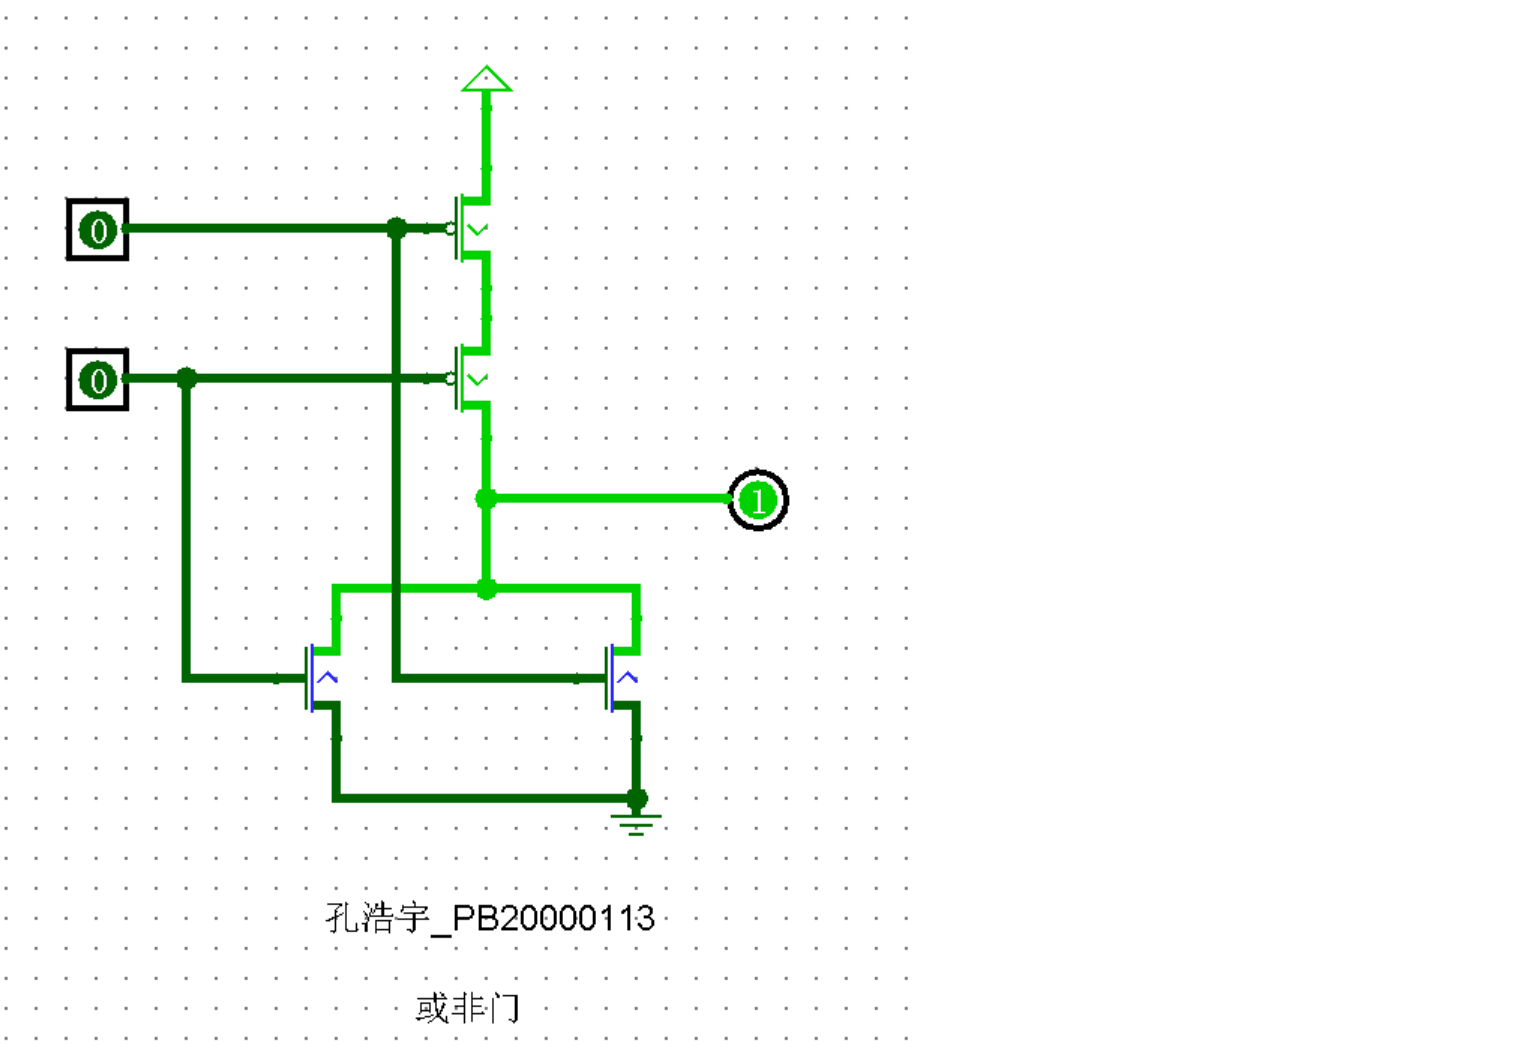
\includegraphics[scale=0.6]{1-3-5.png}
		\end{figure}
		\clearpage
		\subsection*{题目4.}将前面设计的单 bit 与门、或门、非门进行封装,并使用自
		己搭建的三种基本门电路设计一个 1bit 位宽的二选一选择器,统计
		各种基本门的数量。如设计一个 2bit 位宽的四选一选择器,三种基
		本门各需要多少个?
		\begin{figure}[H]
			\centering
			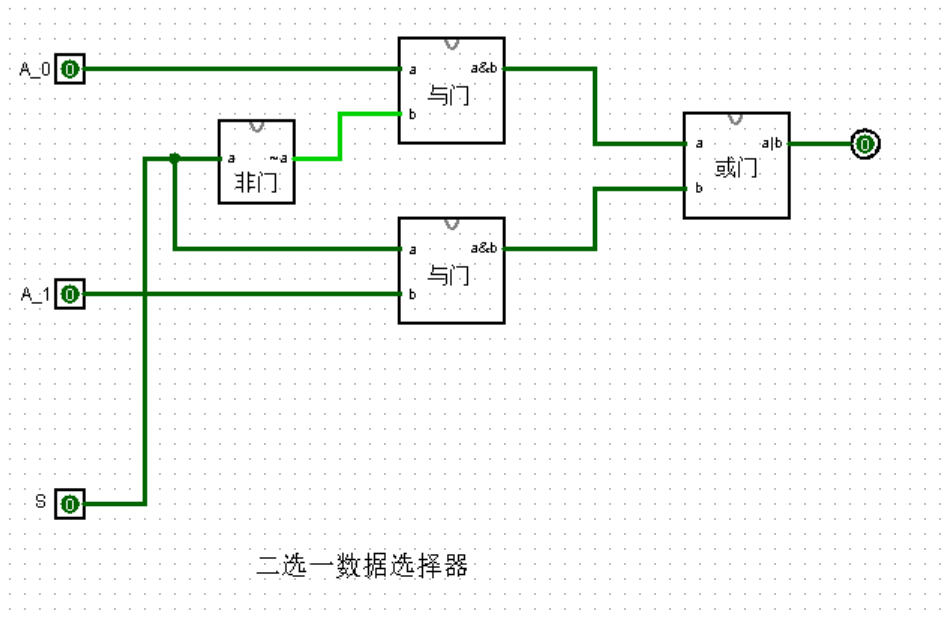
\includegraphics[scale=0.8]{1-4-1.png}
			\caption*{二选一数据选择器}
		\end{figure}
		需要与门2个,非门1个,或门1个。
		\begin{figure}[H]
			\centering
			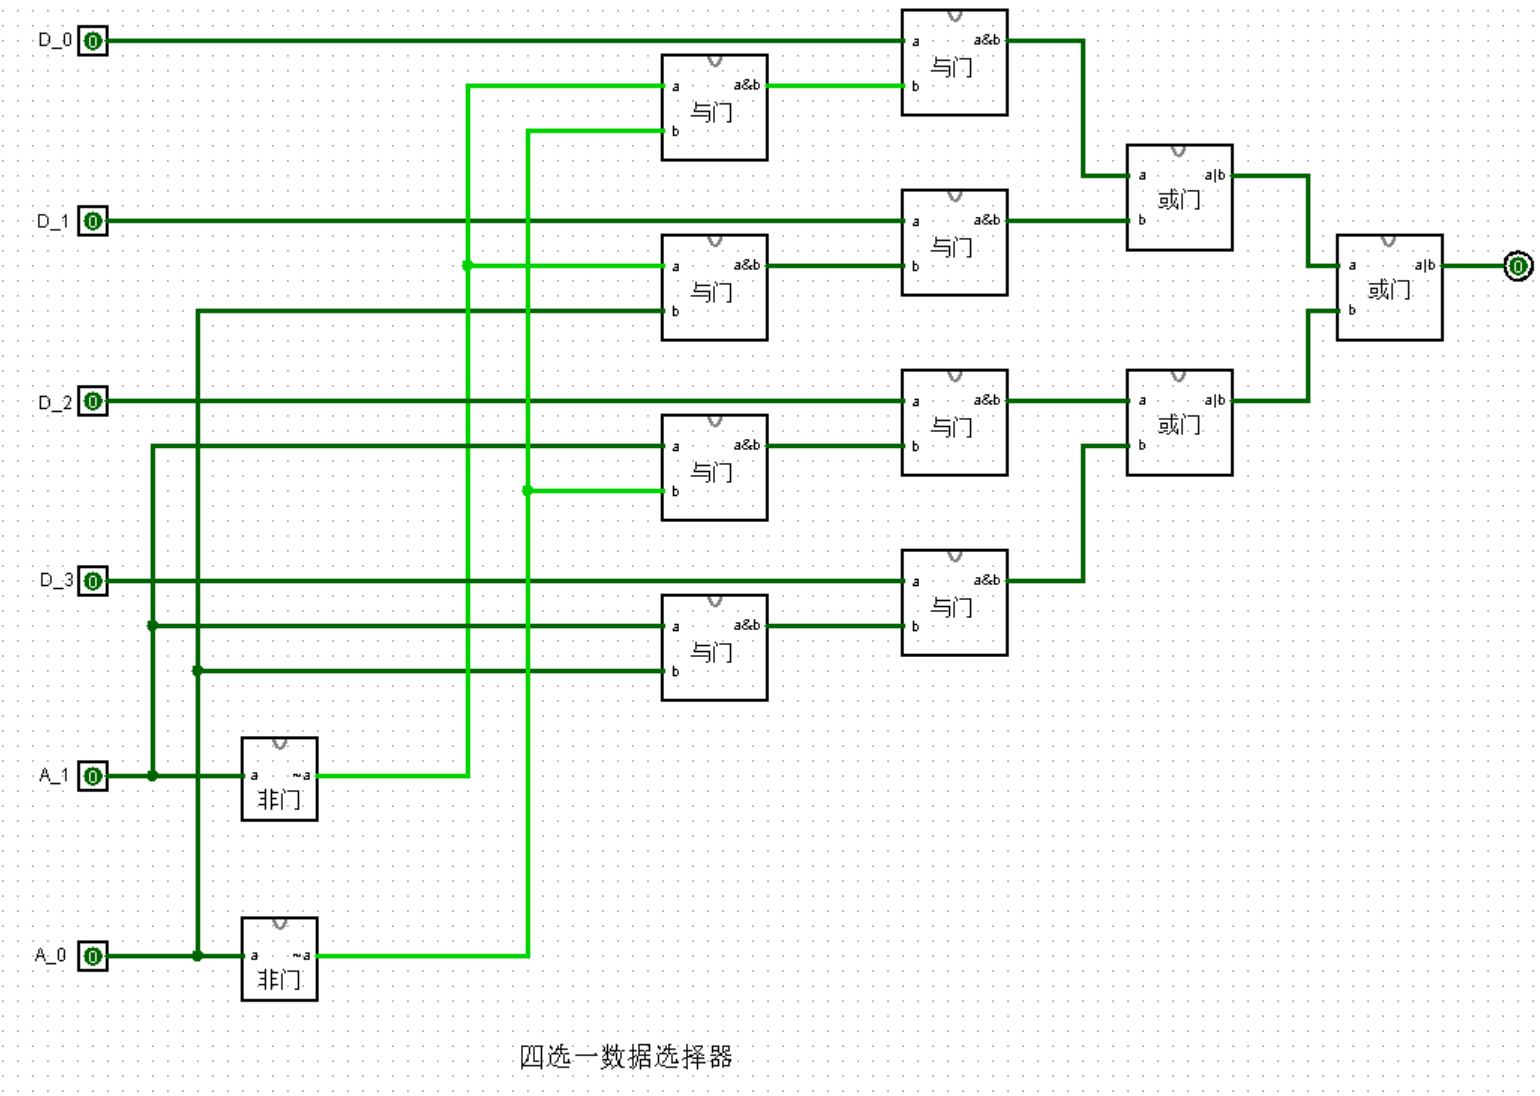
\includegraphics[scale=0.45]{1-4-2.png}
			\caption*{四选一数据选择器}
		\end{figure}
		需要与门8个,非门2个,或门3个。
	\clearpage
    \section{总结与思考}
	\begin{enumerate}
		\item [1.]通过本次实验,初步了解了Logisim,学会了用Logisim搭建简易的逻辑电路,以及电路的封装。
		了解了常量赋值和变量赋值的区别,以及用MOS管搭建逻辑门。
		\item [2.]个人感觉还算比较新手友好的。
		\item [3.]实验不算难,但是前两个实验赋值的时候任务量挺大(主要瞅得眼疼
		\item [4.]可以在实验指导书里面提醒练习1和2用常量赋值。
	\end{enumerate}
\end{document}